\pagestyle{fancy}

\graphicspath{ {Figures/Chapter5_SimulationBenchmarking/} }

In this chapter, several different topics will be addressed. The first two sections present the first benchmarking studies for the PyTT simulation tool. Firstly, we present a measurement performed at LINAC4 in which the thermal evolution of the detectors was indirectly measured and compared to the simulations. These measurements were published in \parencite[][]{ref:IBIC2019ARaceli}. Secondly, we present a comparison between the thermal evolution (for thin wires and thin foil) simulated with PyTT and the commercially available software ANSYS. The following sections present three examples of how the PyTT software has been useful for CERN operation. In particular, we show how the PyTT code has been used to calculate beam power limits at LINAC4 and SPS accelerators. 

\section{Thermionic Measurements at LINAC4}
\label{sec:ThAtLINAC4}

The best way to crosscheck the reliability of the thermal evolution simulations introduced in the previous chapter is to compare them with experimental measurements. Many techniques have been developed for measuring the temperature evolution in objects \parencite[][]{ref:ThMeas1}. In our particular case, we were interested in measuring experimentally the temperature evolution of thin wires ($40 \mu m$) during their interaction with the beam of particles. However, no dedicated setup could be installed in any of the CERN machines. The information available was the intensity registered by the SEM Grids and wire scanners along the LINAC4 accelerator. One can correlate the current measured to the temperature thanks to the thermionic emission process. 

As explained in Chapter \ref{ch:BeamMatterInter}, Section \ref{sec:ThermoCurrent}, Thermionic emission current ($J_{th}$) is negligible at low temperatures but it becomes considerable when higher temperatures are reached. The idea for these measurements was to find certain beam conditions that allowed us to reach high temperatures and thus register the thermionic current. Due to the close relationship between the thermionic current and the temperature, by comparing the simulated current and the experimentally measured one, we could judge the reliability of our thermal simulation results. 

\subsection{Experimental Planning}

For normal beam conditions, the currents measured by the individual wires in SEM grid, or the single wire in a Wire Scanner, are around 1 (mA). For the experimental planning, a signal was considered detectable if the thermionic current was higher than 0.05 (mA). Figure \ref{fig:ThermCurrent} shows the expected current generated, by thermionic emission, in a Tungsten (40$\mu m$) and a Graphite (33 $\mu m$) wire as a function of the wire temperature. From this figure, one can observe that temperatures above 2100 (K) will be required to obtain a detectable thermionic current.  
\begin{figure}[h]
    \centering
    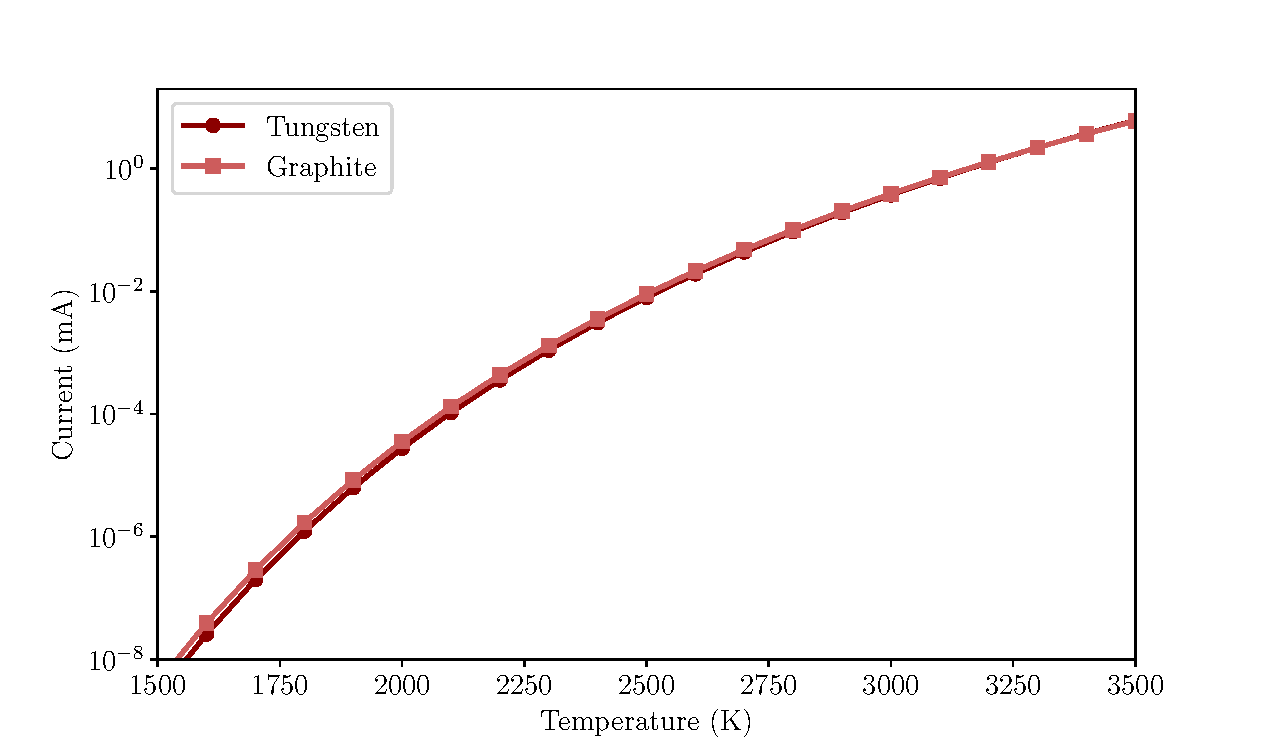
\includegraphics[width=1.0\columnwidth]{Figure_ThermoionicCurrent/ThermoCurrent.pdf}
    \caption{Thermionic current as a function of the temperature for Tungsten (40$\mu m$) and a Graphite (33 $\mu m$) wires.}
    \label{fig:ThermCurrent}
\end{figure}
\begin{figure}[h!]
    \centering
    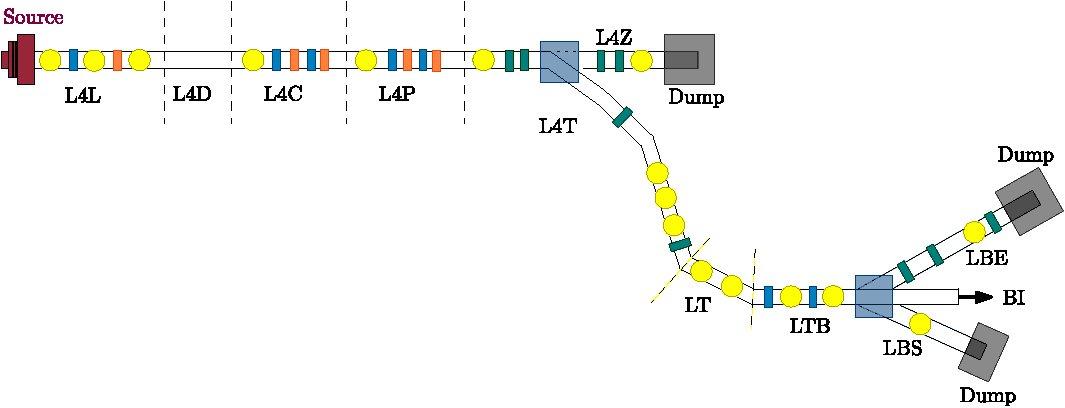
\includegraphics[width=1.0\columnwidth]{Linac4Instrumetnation/Linac4Instruments.pdf}
    \caption{Schematic representation of Linac4 layout, with locations of the SEM Grid (L4T.BSGH/V.0243) and the BCT (L4T.BCT.0107) used for thermionic measurements.}
    \label{fig:DetLocation}
\end{figure}

Due to the high temperatures needed for performing the measurements, the risk of permanent detector damage was non-negligible. Only those detectors with already existing damage, or those placed in areas where it was planned to open vacuum. After some deliberation, it was decided that the SEM grid L4T.BSGH/V.0243, would be used for the measurements. The beam current transformer L4T.BCT.0107 was used for continuous intensity and pulse length measurements. These detectors are located at LINAC4 in the L4T line. The position of these detectors is shown in figure \ref{fig:DetLocation}. 

\begin{table}[h]
    \centering
    \begin{tabular}{cccc}
    \hline
    Pitch   & \# of Wires & Wire Distance (mm) & Covered Region (mm) \\ \hline
    \multirow{5}{*}{3} & 6 + 6 = 12  & 0.4                & 4.4                 \\
                       & 3 + 3 = 6   & 0.75               & 8.9                 \\
                       & 3+3 = 6     & 1.0                & 14.9                \\
                       & 2 + 2 = 4   & 2.5                & 24.9                \\
                       & 2 + 2 = 4   & 4.0                & 40.9                \\ \hline
    \end{tabular}
    \caption{Detailed description of wire location in SEM grid L4T.BSGH/V.0243}
    \label{tab:WireSpacing}
\end{table}
\begin{figure}[h]
    \centering
    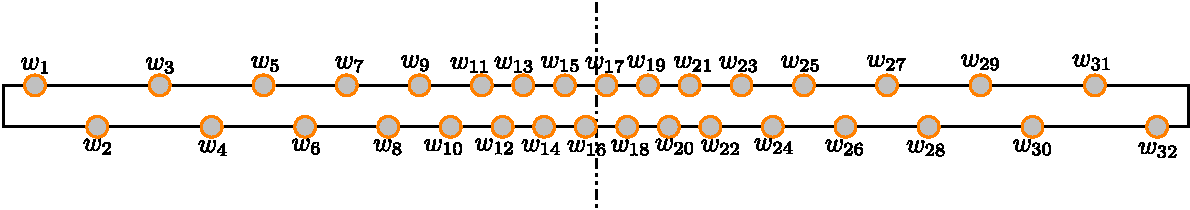
\includegraphics[width=1.0\columnwidth]{Figure_SemGridSchema/SemGridSchema.pdf}
    \caption{Schematic representation of wire position at L4T.BSGH/V.0243. }
    \label{fig:WireSpacing}
\end{figure}

The SEM grid used for the measurement was conformed of 32 Tungsten wires with gold coating. The wires had a length of 5 (cm) and a thickness of 40 $(\mu m)$. The wires were unevenly spaced, covering a total area of 40.9 (mm). Table \ref{tab:WireSpacing} details the locations of the different wires. The wires were placed on the top and the bottom part of the frame alternatively as shown in figure \ref{fig:WireSpacing}.

\begin{figure}[h]
    \centering
    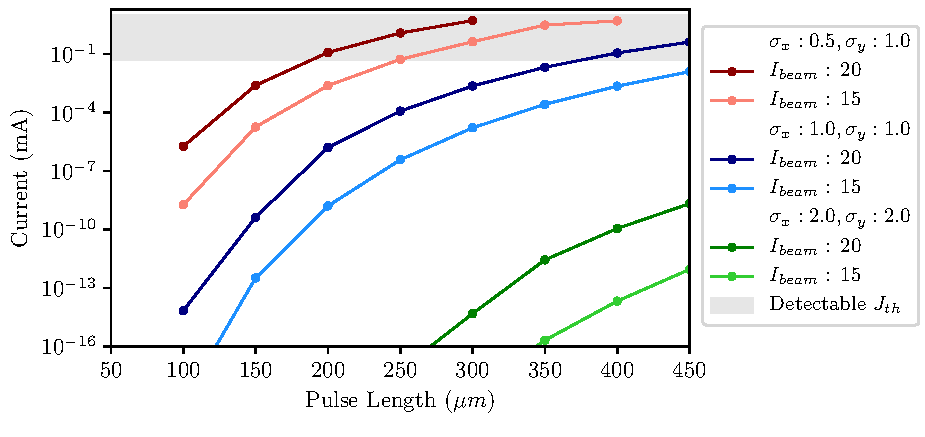
\includegraphics[width=1.0\columnwidth]{Figure_IsThereThermo/IsThereThermo.pdf}
    \caption{Summary of expected maximum current for different beam conditions. Gray Area indicates where thermionic emission is detectable. The beam size is given in (mm) and Beam intensity in (mA).}
    \label{fig:Jth_Cond}
\end{figure}

A preliminary study was performed to determine what kind of beam parameters would potentially yield a detectable thermionic current. In the L4T line, the energy of the \hm beam of particles is already 160 MeV. The beam parameters that could be easily adjusted to convenienceare: Beam intensity ($I_{beam}$), beam pulse length ($\Delta_t$), and beam size ($\sigma_x , \sigma_y$). Figure \ref{fig:Jth_Cond} shows a summary of the maximum expected thermionic current for different beam conditions. 

From this figure one can observe, that large beam sizes ($\sigma_x$ = $\sigma_y$ = 2 mm) will not yield detectable thermionic emission. For smaller beam sizes ($\sigma_x \leq \sigma_y \leq 1$ mm), thermionic emission can be detected for long beam pulse lengths ($\Delta t > 300 $ $\mu s$). Setting up the beam size to a specific dimension is not an easy task. Changes in the intensity of the beam also didn't produce very dramatic changes in the detectable current. During the measurements, these two quantities were kept constant while the beam pulse length was systematically increased in order to reach the thermionic stage in a controlled way. 

\subsection{Experimental Results}

The first set of measurements was taken using conservative beam conditions. The intensity of the beam was kept constant to $I_{beam} = 17.30 (17)$ mA. The beam size was $\sigma_x = 1.02(5) $ mm and $\sigma_y = 1.76(2)$ mm, with the beam centered at $\mu_x = -0.22(6)$ mm and $\mu_y = -0.43(21)$ mm. Figure \ref{fig:PulseEvol} shows the evolution of the beam size and position during a LINAC4 pulse. During these measurements, the beam pulse length was varied between $\Delta t = 165.38(48)$ $\mu s$ up to $\Delta t = 247.12(33)$ $\mu s$. As expected, no sign of thermionic emission was observed. However, when the long beam pulse lengths were measured, wires 15 and 17 were glued together. Figure \ref{fig:WireGlued} shows the current registered by the different wires of the grid as a function of time for four consecutive beam pulses. 

\begin{figure}[h]
    \centering
    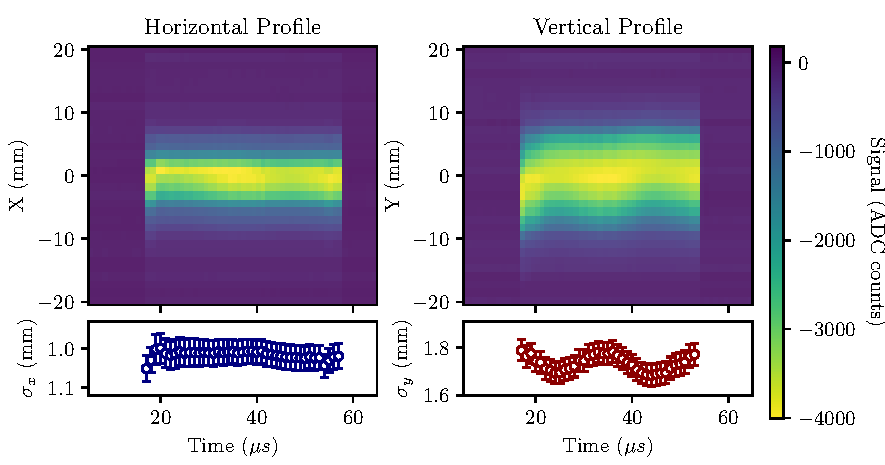
\includegraphics[width=1.0\columnwidth]{Figure_BeamProfileStudy/BeamProfEvol1.pdf}
    \caption{Evolution of the transverse beam profile along the beam pulse. Top: example of transverse beam profile measurement. Bottom: Calculated beam size from gaussian approximation. Error bars were calculated by measuring different beam pulses.  }
    \label{fig:PulseEvol}
\end{figure}

In order to avoid this situation and proceed with the measurements, the beam of particles was steered away from these wires and centered around $\mu_x = -1.89(11)$  $mm$ and $\mu_y = 1.15(31)$ $mm$. The wire separation in this position is much larger, making wire gluing more challenging. The horizontal beam size was reduced to $\sigma_x = 0.59(17) mm$. As a result the vertical plane grew longer, $\sigma_y = 3.23(54)$ $mm$. During these measurements, the beam intensity was slightly smaller $I_{beam} \sim 16.7$ $mA$. The beam pulse length was increased systematically until thermionic emission was observed. On the vertical grid, Thermionic emission was observable in various wires for a beam pulse length of $\sim 450$ $\mu s$. 

\begin{figure}[h]
    \centering
    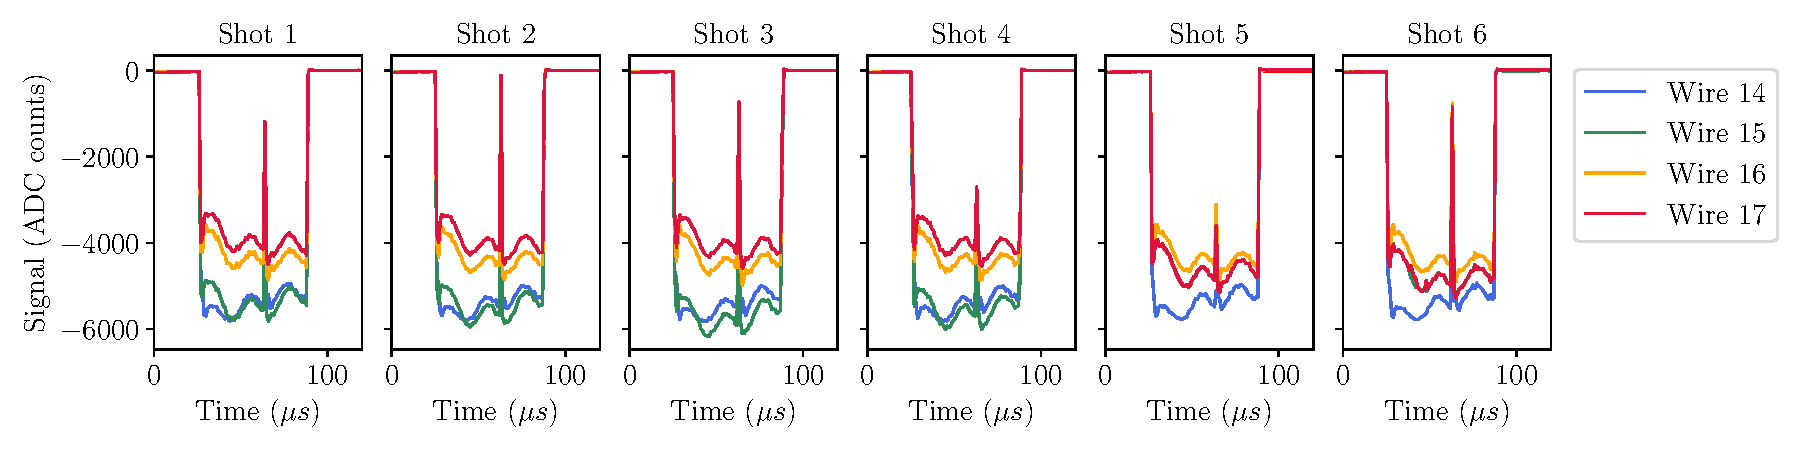
\includegraphics[width=1.0\columnwidth]{Figure_WiresGluing/WireWithTime.pdf}
    \caption{Evolution of the measured current in different wires as a function of time, for six consecutive beam pulses. }
    \label{fig:WireGlued}
\end{figure}
\begin{figure}[h!]
    \centering
    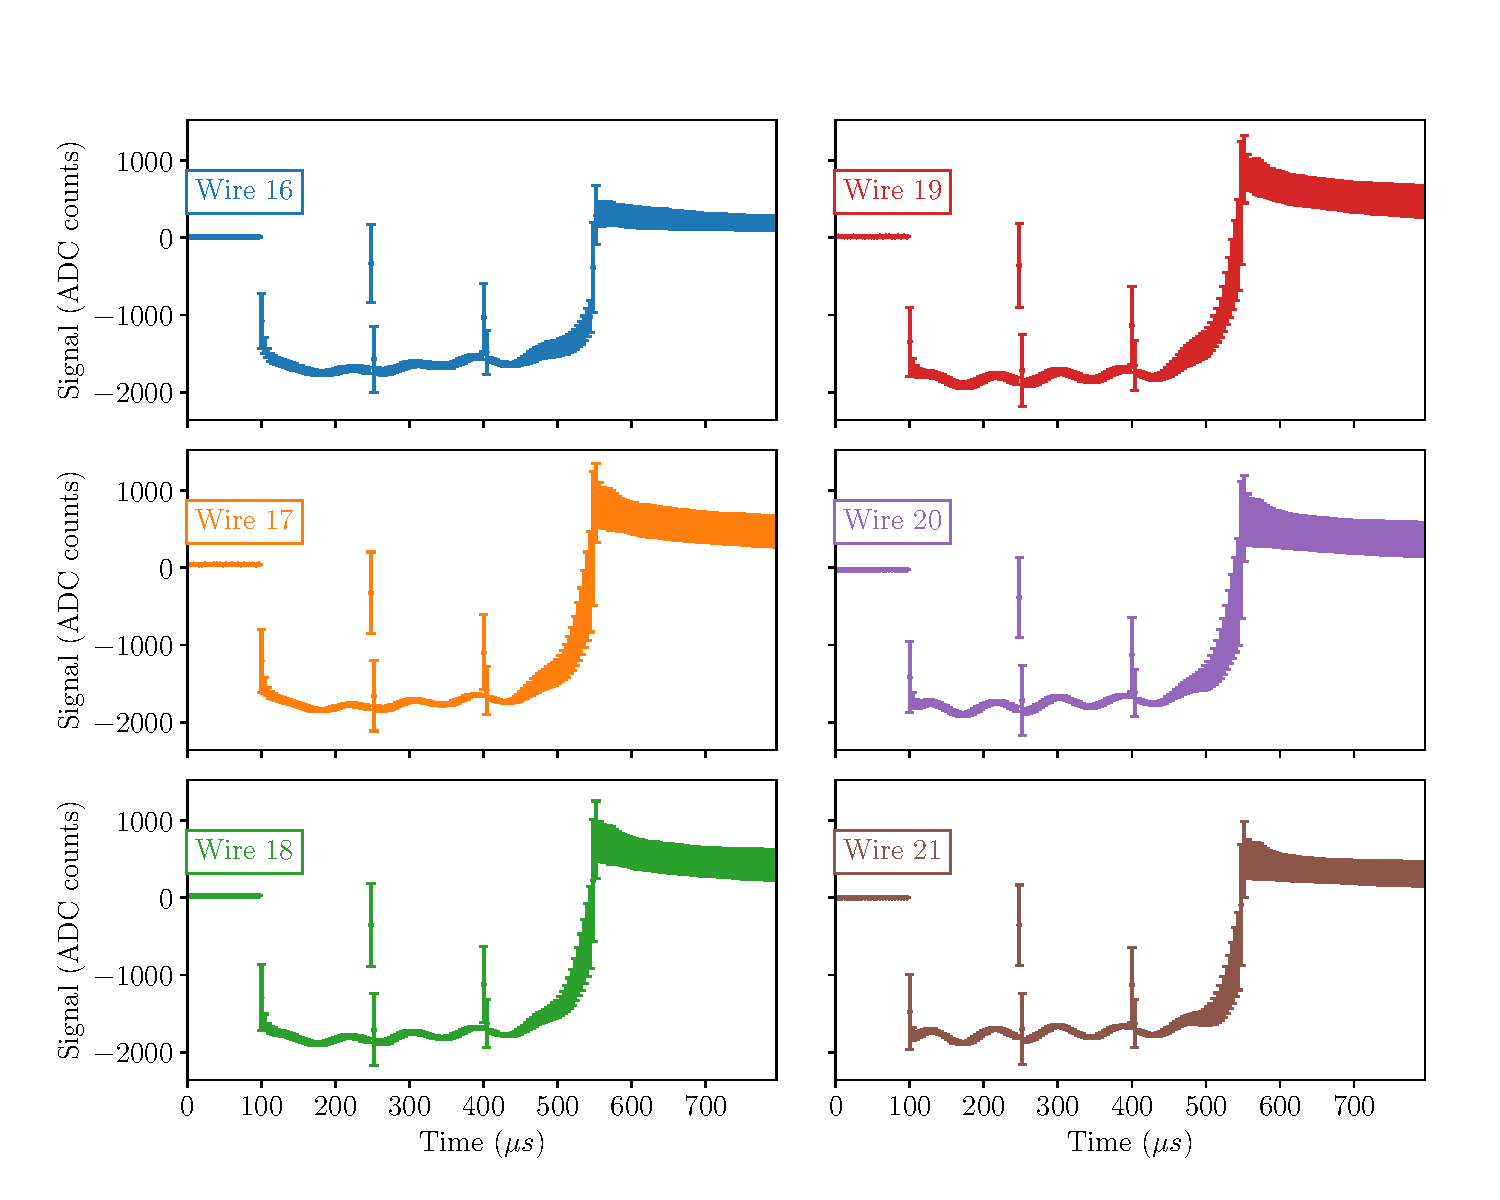
\includegraphics[width=1.0\columnwidth]{Figure_ThermionicMeasurements/VerticalThermoCurrent.pdf}
    \caption{Current registered by several wires during the beam pulse. The units of the signals are (ADC counts).}
    \label{fig:MeasuredThermo}
\end{figure}

Figure \ref{fig:MeasuredThermo} shows the current measured by several wires in the vertical SEM grid during the beam passage. When the particles reached the detector a negative signal is registered. As time goes by, the energy deposition in the detector material rises the temperature of the detector. As temperature increases, thermionic emission increases, and one can observe this increase in the reduction of the absolute value of the current. Once the particle beam has disappeared, a small positive current remains. Because the detector is still warm, thermionic emission current is still being registered.  As the detector cools down, this current diminishes. 

In figure \ref{fig:MeasuredThermo} one can also observe some fluctuations in the registered beam current. This was an effect of the particle beam of particles itself, and could also be observed in the BCT measurements. Also, at $t = 250 \mu s$ and $t = 400 \mu s$, an anomalous value of the beam current is registered by all the wires. To avoid injection losses due to in-between rings injection, the Linac4 chopper removes part of the Linac4 beam every 150 $\mu s$. Which explains the intensity jumps registered by the wires. The intensity fluctuations and gaps at 250 $\mu s$ and 400 $\mu s$, are intrinsic to the particle beam and could also be measured by the BCT. 

The effects of thermionic emission can be also observed in the beam profile measurements. This is shown in figure \ref{fig:JthInProf}. In this figure, lighter currents indicate profiles taken at larger times during the beam pulse. We can see how the beam profile measurements are affected by the thermionic current.

\begin{figure}[h]
    \centering
    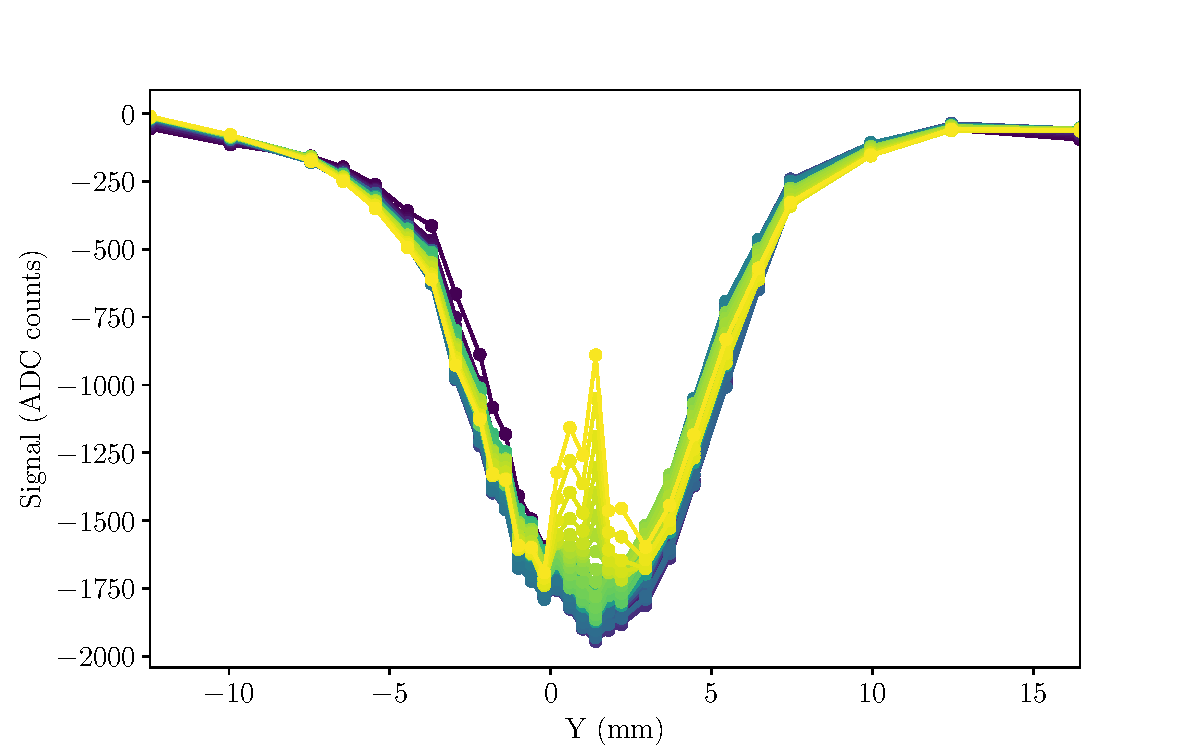
\includegraphics[width=1.0\columnwidth]{Figure_ThermionicMeasurements/ProfileJth.pdf}
    \caption{Example of vertical profile beam measurement. Darker colors indicate measurements at the beginning of the beam shot. Lighter colors indicate measurements a the end of the shot. }
    \label{fig:JthInProf}
\end{figure}

\subsection{Measurment-Simulation Comparison}

% PyTT program was used to simulate the thermal and electrical evolution of the detectors during the measurements. For the simulations, the intensity of the beam was considered to be constant. Intra-pulse intensity fluctuations and chopper effects were not considered. Figure \ref{fig:MeasSimCompa} shows a comparison between the signal measured by wire 19 of the SEM grid, the simulated current, and the current measured by BCT.0107. The BCT intensity has been included in the comparison to show the intrinsic properties of the beam. The BCT signal clearly shows when the Beam pulse starts and ends. It also shows the aforementioned beam intensity fluctuations and the chopper gaps. However, the current reduction at longer beam pulse time is not observable in the BCT measurements, as this is an effect occurring on the wire. 

% \begin{figure}[h]
%     \centering
%     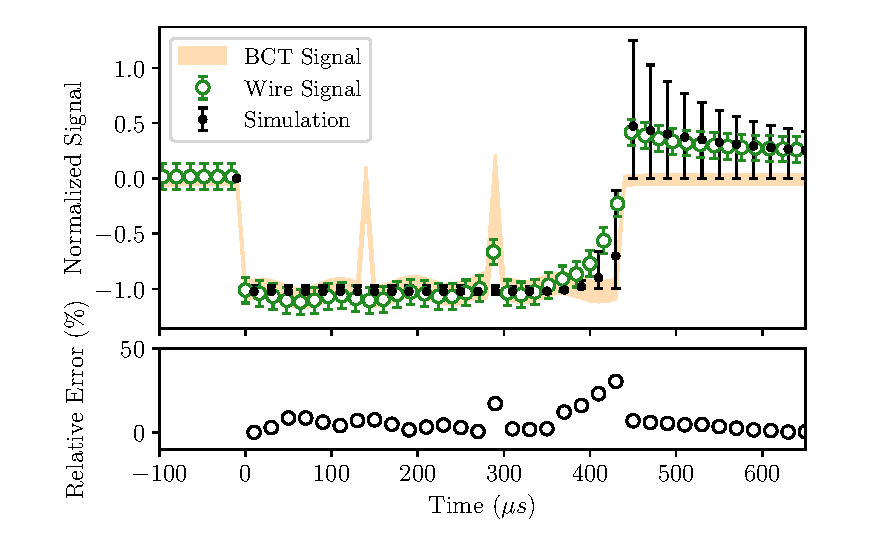
\includegraphics[width=1.0\columnwidth]{Figure_MeasurementSimulationCompa/VerticalCompa.pdf}
%     \caption{Signal generated in the wire intercepting the beam as a function of time. Compared with simulated intensity results. }
%     \label{fig:MeasSimCompa}
% \end{figure}

%  Also, the positive current used by the wire after the beam pulse has passed is not observable in the BCT signal. This means the current measured by the detector at that time does not come from the beam. The simulation results seem to very clearly reproduce the average of the measured SEM current. The simulations show a slightly slower start for the thermionic emission current. However, after the beam pulse is gone, the simulated and the measured results for the thermionic current match very well. 

% The maximum relative error between simulated and measured results is found to be around 30 $\%$, and it is found at the very end of the beam shot. Even then, the average relative error along the whole pulse is $6.3(25) \%$. 

% A dedicated uncertainty study was performed to determine the uncertainties of the simulated results (See Section \ref{sec:ModelUnc}). In this particular case, the biggest contributor to the simulation's uncertainty came from uncertainties in the beam size. As indicated in the previous section, the beam size was $\sigma_x = 0.59(17)$ mm and $sigma_y = 3.23(54)$ mm. This implies, beam size uncertainty was $\xi_x = 28.81 \%$ and $\xi_y = 16.71 \%$. As shown in section \ref{sec:ModelUnc}, uncertainties in beam sizes can yield big uncertainties in simulation results, mainly when small beam sizes are involved. 

% As we saw in figure \ref{fig:MeasuredThermo}, several wires measured thermionic emission. However, due to the small changes in the measured intensity between the different wires and the big uncertainties in the simulated results, it was impossible to distinguish among them. 


% \section{Simulation Comparison: Ansys}
% \label{sec:AnsysComparison}

% The objective of this study was to compare the results obtained with the PyTT code, with results obtained with Ansys, a highly used and benchmarked commercially available software. 

% For this work, the theory of finite differences (FDM) has been used to solve the heat equation, as was explained in Chapter \ref{ch:TempModeling}. However, FDM is just an example of a numerical technique to solve PDEs and it is important to stress that alternative approaches abound. Commercially available softwares, such as Ansys \parencite[][]{ref:Ansys}, are commonly used to accurately solve a big variety of multiphysics phenomena. In particular, Ansys uses Finite Element Analysis (FEA) \parencite[][]{ref:NumericalMethodBook} to aid the users obtain solutions for real engineering problems. 

% \subsection{Thin Wire Studies}

% The first part of this study compares the thermal evolution results, of a thin tungsten wire ($\phi$ = 40 $\mu m$), calculated with the PyTT code and Ansys. Here, a LINAC4-like beam of particles was considered as the heating source. Table \ref{tab:BeamParametersCompa} summarizes the parameters of the beam. The parameters on this table remained constant for all the simulations. The beam pulse length was systematically varied to cover different temperature ranges. 

% \begin{table}[h]
%     \centering
%     \begin{tabular}{ccccc}
%     \hline
%     Particle & \begin{tabular}[c]{@{}c@{}}Energy\\ (MeV)\end{tabular} & \begin{tabular}[c]{@{}c@{}}Inensity\\ (mA)\end{tabular} & \begin{tabular}[c]{@{}c@{}}Sigma x \\ (mm)\end{tabular} & \begin{tabular}[c]{@{}c@{}}Sigma y\\ (mm)\end{tabular} \\ \hline
%     Proton   & 160   & 25      & 0.5           & 1.                        \\ \hline
%     \end{tabular}
%     \caption{Summary of the beam parameters that remained constant during the simulations.}
%     \label{tab:BeamParametersCompa}
% \end{table}

% \begin{figure}[h]
%     \centering
%     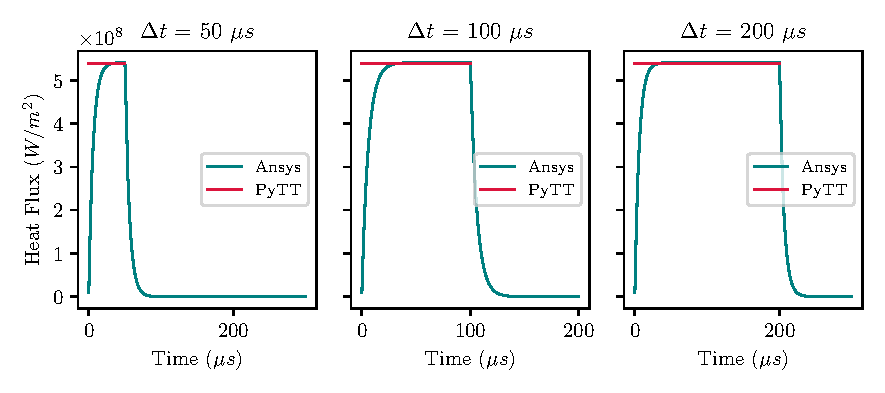
\includegraphics[width=1.0\columnwidth]{HeatInpuCompa/HeatInputCompa.pdf}
%     \caption{Examples of the heat flux provided to Ansys and PyTT for three different simulation cases.}
%     \label{fig:AppliedHeatWire}
% \end{figure}

% To achieve the closes simulation conditions, a cuboid approximation of the wire was considered in both, PyTT and Ansys. The wire was oriented along the y-axis, with a wire length of 2 (cm). The spatial mesh resolution was 0.1 (cm) along the wire length and for the x and z directions a single mesh element was considered. The temporal resolution was divided into two sections. During the beam pulse, temporal elements of $10^{-7}$ (s) were considered, while during the cooling section the temporal elements were $10^{-4}$ (s) long. Material parameters, such as heat capacity and conductivity, were considered to be temperature-dependent. However, the emissivity was considered to be constant and equal to 0.1 in both cases. 

% In Ansys, the heat load was given using APDL commands \parencite[][]{ref:APDLCommand}. Here, a gaussian distribution with the heat flux ($W/m^2$) equivalent of a beam pulse was described and applied to the material surface. Figure \ref{fig:AppliedHeatWire} shows the heat flux applied to the wire by both Ansys and PyTT. The heat load in PyTT is constant during the presence of the beam pulse, and it immediately goes to zero once the beam pulse has passed. In the case of Ansys, a more smooth heat load transition is observed. The total integrated heat flux was the same in both programs, with a maximum discrepancy of $0.64\%$ for the shorter beam pulses ($\Delta t \leq 50$ $\mu s$). 

% Figure \ref{fig:TemperatureComparison} compares the evolution of the maximum temperature, for three different beam pulse lengths, as a function of time. In these figures, one can observe how the PyTT simulations systematically give a higher maximum temperature than the results obtained with Ansys. The cooling rate in the PyTT code seemed to be slightly slower than in Ansys. The maximum discrepancy between the Ansys and the PyTT results was $11.2\%$ for a temperature of 1356K. 

% \begin{figure}[h]
%     \centering
%     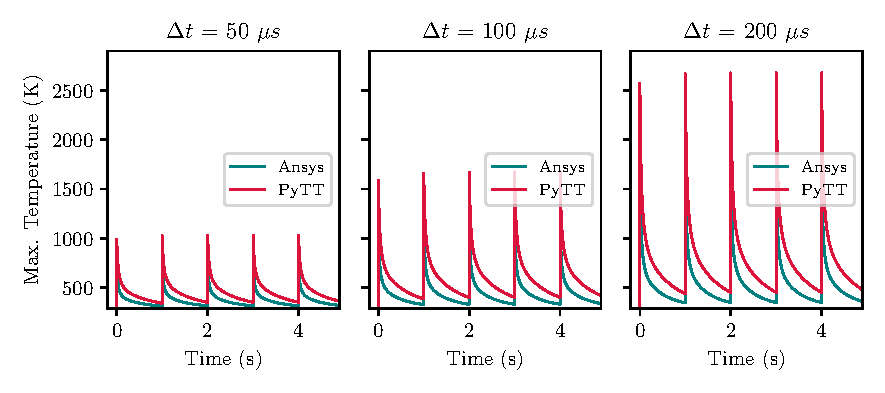
\includegraphics[width=1.0\columnwidth]{TempCompa/TempCompa.pdf}
%     \caption{Comparison of the evolution of the maximum temperature in the detector as a function of time, for three different beam pulse lengths.}
%     \label{fig:TemperatureComparison}
% \end{figure}

% One big difference between these two programs when performing this study was the simulation time. PyTT averaged 10.56 (s) when performing these simulations, while Ansys averaged 7:35 (min), in a Hp Intel(R) Core(TM) i7-6700 CPU, 16.0 Go RAM. This comparison might not be fair, Ansys is a much more complex simulation tool, with many many more options and accurate models. Also with the appropriate knowledge, the simulation times can be optimized. However, if what is important is to quickly obtain a number that can give the user if certain beam parameters are going to damage or not a detector, the PyTT code can manage to do it fast, with results that are very similar to the ones obtained with Ansys. 

% \subsection{Thin Foil Studies}

% Similar Studies were performed with thin graphite foils ( dimensions = 2 (cm) x 2 (cm) x 40 ($\mu m$)). The beam conditions for this study were the same as the ones described in table \ref{tab:BeamParametersCompa}. Variations on the beam pulse length were used again to control the maximum temperature reached by the detectors. 

% \begin{figure}[h]
%     \centering
%     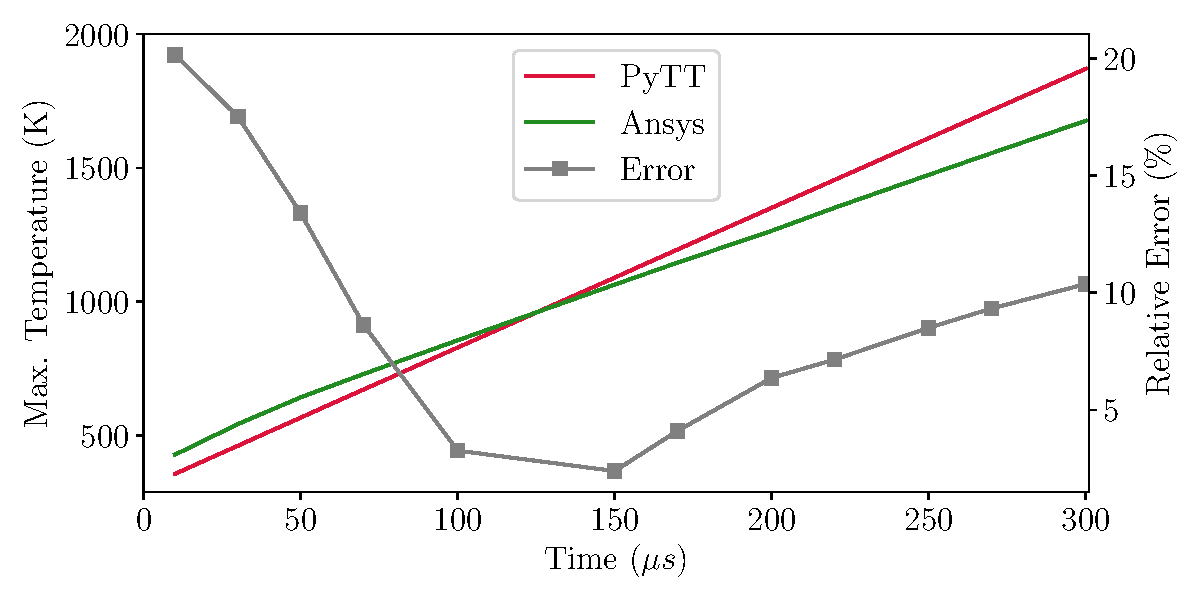
\includegraphics[width=0.9\columnwidth]{ErrorCompa/FoilMaxTempCompa.pdf}
%     \caption{Comparison of the evolution of the maximum temperature in $40 \mu m$ graphite foil, as a function of beam pulse length. On the right axis, the relative error between them is represented. }
%     \label{fig:TempMaxErrCompa} 
% \end{figure}
% \begin{figure}[h]
%     \centering
%     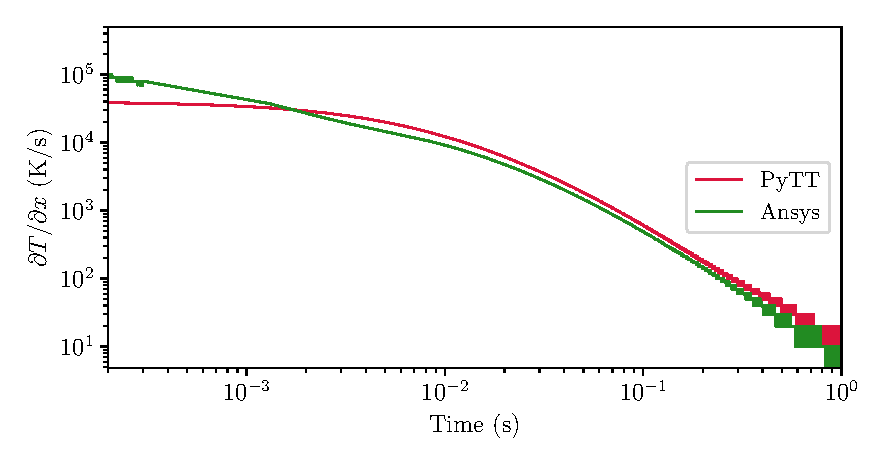
\includegraphics[width=0.9\columnwidth]{CoolingSpeedAnsys/CoolingSpeed.pdf}
%     \caption{Comparison of the cooling rate between PyTT code and Ansys. For a $40 \mu m$ graphite foil after a beam shot. }
%     \label{fig:CoolingRate} 
% \end{figure}

% Figure \ref{fig:TempMaxErrCompa} shows the maximum temperature reached (at equilibrium), with both PyTT and Ansys codes, as a function of the beam pulse length. From this figure, one can see how at higher temperatures PyTT continues to systematically give a higher maximum temperature. However, at lower temperatures, Ansys gives higher temperature results. The relative error between the Ansys and PyTT results is higher at lower beam pulse lengths, however, it never exceeds a $20 \%$.

% For a beam pulse length of $100$ $\mu s$, the cooling rate was calculated with Ansys and with PyTT. Figure \ref{fig:CoolingRate} shows a comparison between the cooling rate after a beam shot. From this figure, we can observe how Ansys presented a much faster cooling at the beginning (higher temperatures) and a slower cooling after some time (lower temperatures). Here, the temperature right after the beam shot was 848 (K).

% Another interesting feature we wanted to compare was the heat distribution in space. Figure \ref{fig:FancyPlotComparison} shows the heat distribution of the foil simulated with Ansys (left) and the PyTT code (right). These two figures were taken at the same instant of time (10 ms after beam shot arrival), during the cooling process. It is clear from these pictures that the heat distribution is very similar in both cases. It is very difficult to properly understand the differences between these results. Information about the numerical methods employed by Ansys is not publicly available. So no more quantitative or in-depth conclusions could be taken from these studies. 

% \begin{figure}[h]
%     \centering
%     \begin{subfigure}[b]{0.6\textwidth}
%         \centering
%         \includegraphics[width=\textwidth]{AnsysPyTT_2Dcompa/Ansys2DPlot.png}
%     \end{subfigure}
%     \hfill
%     \begin{subfigure}[b]{0.8\textwidth}
%         \centering
%         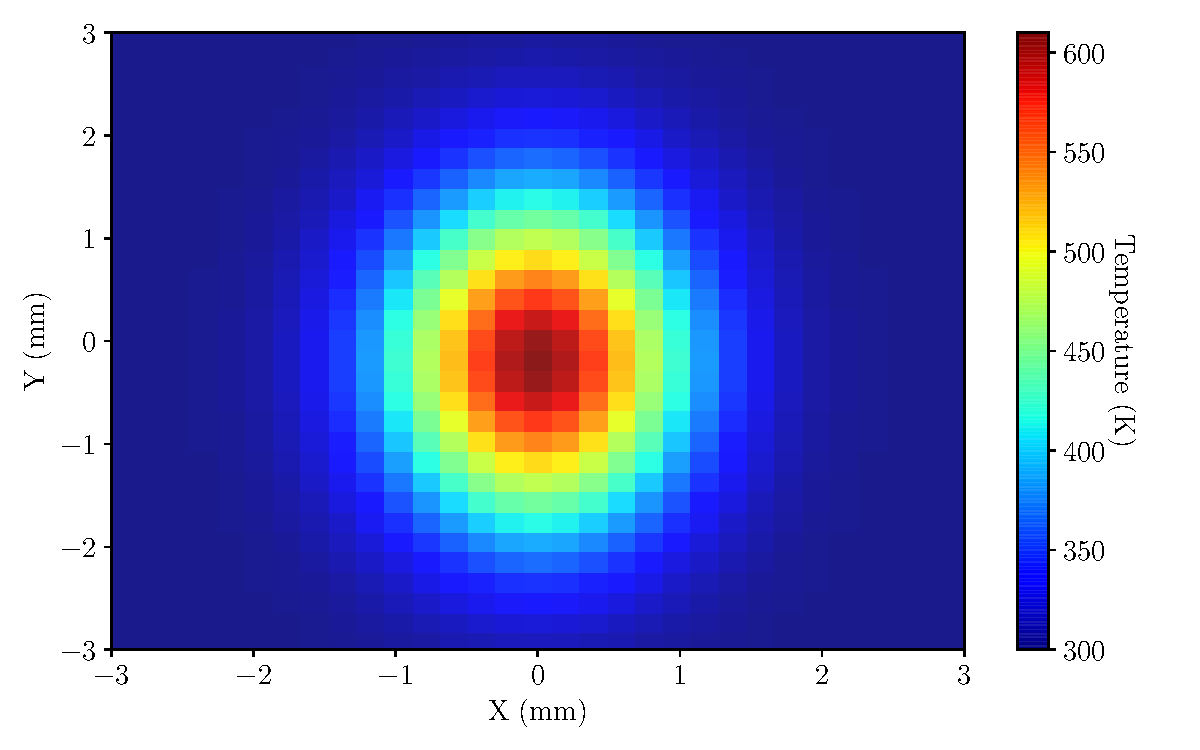
\includegraphics[width=\textwidth]{AnsysPyTT_2Dcompa/FoilPyTT.pdf}        
%     \end{subfigure}

%     \caption{Comparison between thermal distribution in Graphite foil after one beam shot. In Ansys (top) and PyTT code (bottom). The black lines in Ansys have a separation of 1 mm.}

%      \label{fig:FancyPlotComparison} 
% \end{figure}

% \section{Beam Power Limit Calculations}

% Determining beam power limits means determining beam conditions that could potentially damage the detectors. To do that, the PyTT program was used to simulate the maximum temperatures reached by the detectors for the different expected beam conditions at their location. If the maximum temperature reached was above the safe limit, those beam conditions were considered to be harmful to the detectors. 

% \subsection{SEM grid and Slow Wire Stanner at Linac4}
% \label{sec:BeamPowerL4}

% For Linac4, the beam conditions under study were: Beam Intensity ($I_{beam}$), beam pulse length ($\Delta t$) and beam size ($\sigma_x , \sigma_y$). Figure \ref{fig:DetLocation} shows a schematic representation of Linac4, with the different detectors location. The detectors in the L4L, L4D and L4C lines are made of graphite wires (33 $\mu m$). The rest of the wire scanner detectors are also graphite wires, whereas the SEM grid detectors are gold-coated tungsten wires (40 $\mu m$). Table \ref{tab:beamprop} summarizes the range of the beam properties expected along the Linac4 accelerator.

% For each detector, a set of dedicated simulations covering the whole parameter range were performed with the PyTT program. A maximum temperature of 1400K was taken as a safe maximum temperature limit. This limit is probably very conservative, as most of the detectors could easily handle up to 3000 K. However, due to the wire-gluing problem suffered in SEM grid detectors, due to gold coating, a much lower temperature limit was established. 

% \begin{table}[h]
%     \centering
%     \begin{tabular}{cccc}
%     \hline
%     Property                          & Min & Max & Units   \\ \hline
%     Intensity ($I_{beam}$)            & 10  & 25  & mA      \\
%     Pulse Length ($\Delta t$)         & 50  & 400 & $\mu s$ \\
%     Beam Size ($\sigma_x , \sigma_y$) & 0.5 & 3.0 & mm      \\ \hline
%     \end{tabular}
%     \caption{Range of beam properties expected at Linac4 accelerator.}
%     \label{tab:beamprop}
% \end{table}

% Figure \ref{fig:EnerCompa} shows an example of the power limits calculated for a detector in L4C line (Detector 5) and a detector at the L4T line (Detector 12). Each square represents the maximum temperature reached by a simulation with the beam pulse length indicated on the X-axis, and the beam intensity indicated on the Y-axis. The beam size in both cases was $\sigma_x = \sigma_y = 2.0$ mm. In both cases, we can observe that beam pulse lengths smaller than 200 $\mu s$ are very safe. Neither detector was getting close to the set temperature limit. The only difference between the detectors is the energy deposition in the material. At higher energies, the energy deposition is smaller, so the maximum temperatures reached by the detector are smaller than the equivalent conditions at lower energies. 

% Figure \ref{fig:SigmaComparison} shows a similar set of results, but this time, both detectors were placed at locations where the particle energy was already 160 MeV. The difference between the right plot and the left plot is the beam size. The left-hand side figure pictures a small beam size. The right-hand side figure pictures a larger beam size. From this figure, we can observe how small beam sizes result in much more critical thermal conditions. 

% In general, one should be very careful measuring small beam sizes at low energy ranges. An overall power limit for the Linac4 accelerator was established. Beam conditions were considered to be dangerous if the beam size was smaller than 1 $(mm)$ and the beam pulse length was longer than $100 ()\mu s)$. An interlock system for SEM grids and wire scanners was established at Linac4 based on these results. 

% \begin{figure}[h]
%     \centering
%     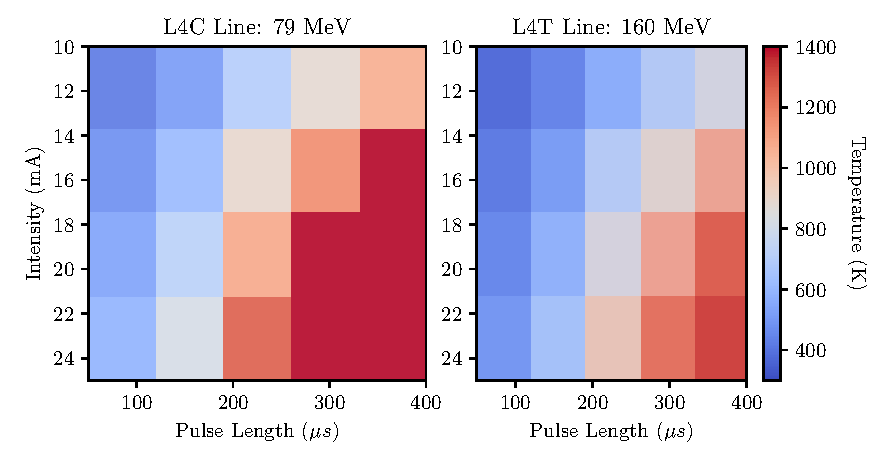
\includegraphics[width=1.0\columnwidth]{Figure_ThermalLimitsSquares/EnergyCompa.pdf}
%     \caption{Power limit calculations for a detector at L4C (Left) and a detector at L4T (right) lines. The beam size in both cases was $\sigma_x = \sigma_y = 2.0$ mm.}
%     \label{fig:EnerCompa}
% \end{figure}

% \begin{figure}[h]
%     \centering
%     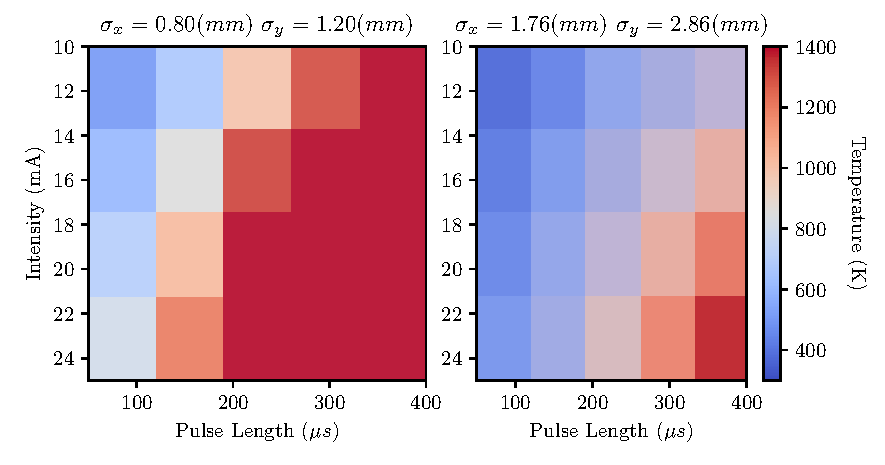
\includegraphics[width=1.0\columnwidth]{Figure_ThermalLimitsSquares/SigmaCompa.pdf}
%     \caption{Power limit calculations for a detector at 160 MeV beam energies.}
%     \label{fig:SigmaComparison}
% \end{figure}

% \subsection{Fast Wire Scanners at SPS}
% \label{sec:BeamPowerSPS}

% A new generation of beam wire scanners has been developed at CERN, in the framework of the LIU project \parencite[][]{ref:WireScanJose}. In the SPS, 4 new wire scanner systems were installed, for horizontal and vertical beam size measurements. In this case, the relevant parameters under study were: beam emittance (at injection and extraction), the number of protons per bunch (from $10^9$ to $10^{11}$), the maximum number of bunches (from 1 to 288) and wire scanner velocity (form 1 m/s to 20 m/s). 

% For the SPS energies ( 26 GeV at injection and 450 GeV at extraction ) differences in energy deposition are not as important as in the Linac4 case. Beam sizes are still a very important parameter to consider. In the SPS, the beam size is usually described in terms of beam emittance. One can easily convert from one to the other with the following relation: 

% \begin{equation}
%     \sigma = \sqrt{\frac{\epsilon_{norm}}{\gamma_{rel} \cdot \beta_{rel}} \cdot \beta(s)}
% \end{equation}

% Where $\epsilon_{norm}$ refers to the normalized emittance and $\beta_{rel}$, $\gamma_{rel}$ are the relativistic parameters. $\beta(s)$ is the courant-Snyder parameter at the position s. However, because the beam size decreases as the relativistic parameters increase, smaller beam sizes are found in the extraction case. 

% \begin{figure}[h]
%     \centering
%     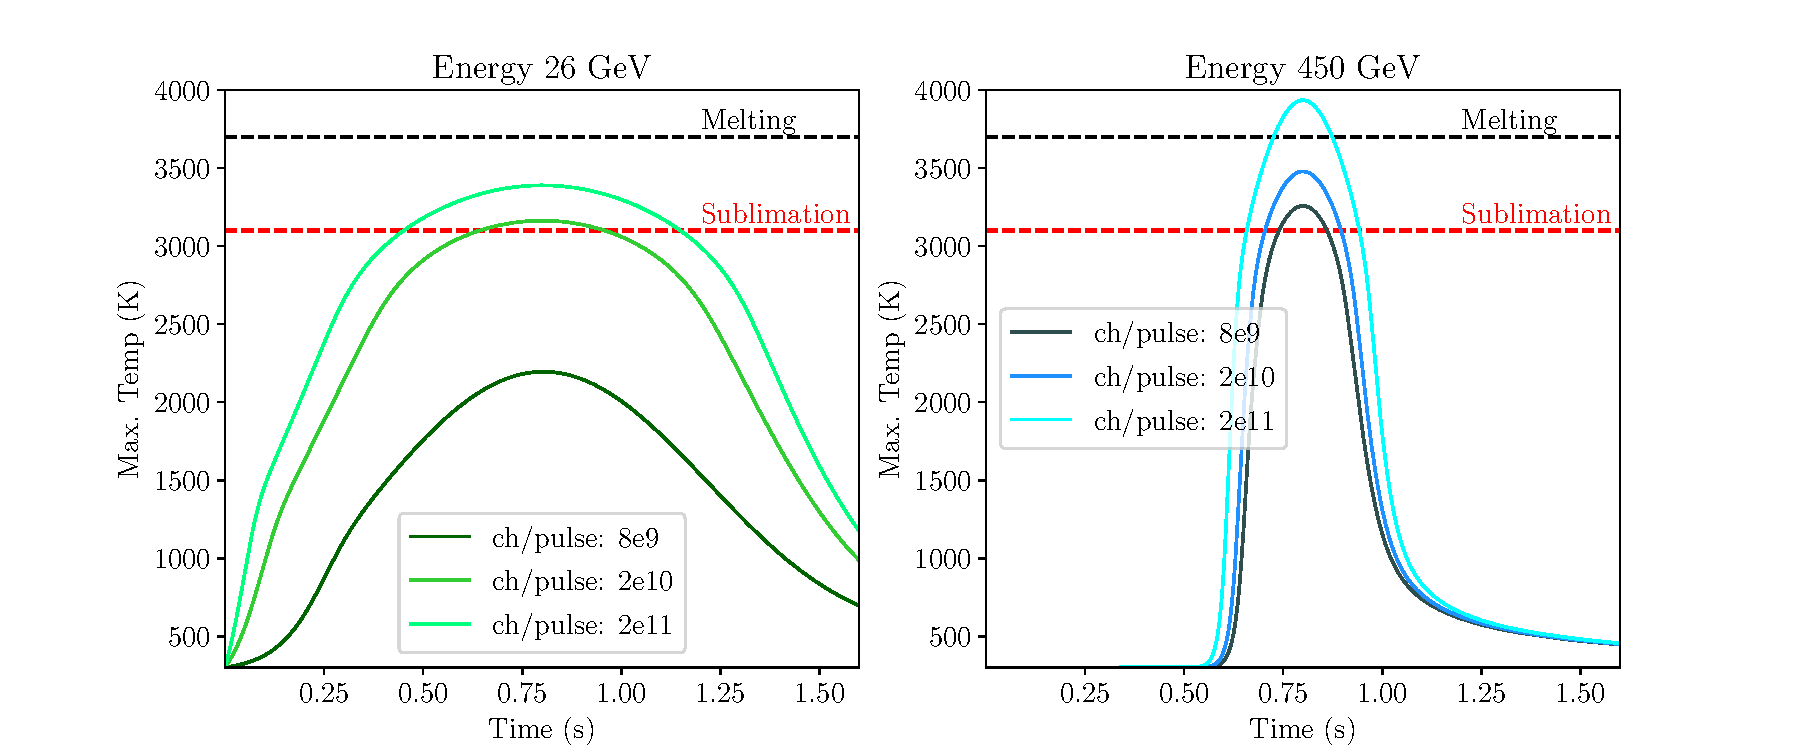
\includegraphics[width=1.0\columnwidth]{WireScanner_Limits/WireLim1.pdf}
%     \caption{Comparison of maximum fast wire scanner temperatures reached for different beam conditions. Left: Injection energy. Right: Extraction energy.}
%     \label{fig:WireScanner1}
% \end{figure}

% Figure \ref{fig:WireScanner1} shows the evolution of the maximum temperature reached by a 33 $\mu m$, graphite, fast wire scanner for a different number of particles per bunch. In this figure, the wire scanner speed was set constant to 1 m/s, and the total number of bunches was always 288.  The figure on the left is for injection energies (26 MeV) and the one on the right is for extraction energies (450 MeV). In both cases, the higher the number of particles per pulse the higher the temperature reached by the detector. In these figures, we can also see the decrease of the beam size with the energy, as the temperature increase happens in a much narrower period during extraction energies. 

% The wire velocity is also a very important factor to consider. The slower the wire velocity the longer time it will spend in the central area of the beam, and thus the higher the maximum temperature reached. Increasing the wire speed is beneficial in terms of thermal limitations. However, as a tradeoff, we have the measurement resolution. Because the wire scanner in the SPS is much slower than the bunches being accelerated (revolution period $t_{rev} = 2.4\cdot 10^{-5} s$). The number of points per sigma taken by a fast wire scanner can be calculated as: 

% \begin{equation}
%     n_{points} = \frac{\sigma}{v_{w}\cdot T_{rev}}
% \end{equation}

% For a beam size of 1 mm, a maximum speed of 10 m/s can be used. Otherwise, the measurements would not have enough resolution. The wire damage can be associated with the density of charges traversing the wire \parencite[][]{ref:Msapinski}:

% \begin{equation}
%      n_{ch} = \frac{N_{ch} \cdot d_{w}}{v_{w} \cdot t_{rev} \cdot \sigma}
% \end{equation}

% Where $N_{ch}$ is the total number of particles, understood as the number of particles per pulse times the number of pulses. $d_w$ is the wire diameter and $v_w$ is the wire velocity. As a limiting scenario, we could consider the case of a 33 $\mu m$ Graphite wire, with a speed of 1 m/s and measuring a beam size $\sigma_x = \sigma_y = 0.3$ mm. In this case the density of particles $n_{ch} = 2.5\cdot 10^{12}$. Beam and wire conditions yielding a charge density higher than this number, are considered to be potentially harmful.

% This number is consistent with the experiments performed by M. Sapnski \parencite[][]{ref:Msapinski}. This value is used in the SPS accelerator as a safety limit. Table \ref{tab:MaxNturns} shows an example of how this safety value was used to calculate the maximum number of allowed turns for different wire scanners and beam conditions. At CERN SPS, the maximum number of injected turns can go up to 288. From this table, we can observe that only at injection energies this number of bunches can be measured. 

% \begin{table}[h]
%     \centering
%     \begin{tabular}{cclccccc}
%     \hline
%     \multirow{2}{*}{\begin{tabular}[c]{@{}c@{}}Energy \\ (GeV)\end{tabular}} & \multicolumn{2}{c}{Beam Size (mm)} & \multicolumn{5}{c}{Wire Velocity (m/s)} \\ \cline{2-8}    & $\sigma_x$               & $\sigma_y$              & 1     & 6      & 10    & 15    & 20     \\ \hline
%     \multirow{2}{*}{25}                                                      & 3.03             & 2.10            & 54    & 323    & 538   & 807   & 1080   \\
%      & 2.0              & 1.38            & 35    & 213    & 350   & 531   & 708    \\ \hline
%     \multirow{2}{*}{450}   & 0.72             & 0.50            & 12    & 74     & 129   & 194   & 258    \\    & 0.47             & 0.33            & 8     & 51     & 85    & 127   & 170    \\ \hline
%     \end{tabular}
%     \caption{Maximum allowed number of beam bunches for different beam conditions. The number of charges per bunch was $1.5 \cdot 10^{11}$ ch/bunch. }
%     \label{tab:MaxNturns}
% \end{table}

